% GitTalk
% Copyright 2010 Wähnert
% E-Mail: waehnert@mis.mpg.de
%
% This work is licensed under the Creative Commons 
% Attribution-Noncommercial-Share Alike 3.0 Germany License.
% To view a copy of this license, visit 
%
%   http://creativecommons.org/licenses/by-nc-sa/3.0/de/
%
% or send a letter to Creative Commons, 171 Second Street,
% Suite 300, San Francisco, California, 94105, USA.
\documentclass{beamer}
\usepackage[english]{babel}
\usepackage{graphicx}
\usetheme{Torino}
\usecolortheme{crane}
\usepackage{lastpage}
%\usepackage{beamerthemesplit}
%\usepackage{listings}

%\lstset{numbers=left, numberstyle=\ttfamily, numbersep=1ex, xleftmargin=0.5cm, %
%columns=fixed, basewidth=1.2ex, basicstyle=\ttfamily, showstringspaces=false, aboveskip=\smallskipamount, %
%belowskip=\smallskipamount}
%\lstset{language=bash}
%\renewcommand*{\thelstnumber}{\$}

\setcounter{tocdepth}{1}

\title{Git - A distributed version control system}
\author{Philipp W\"ahnert}
\institute{Max Planck Institute for Mathematics in the Sciences}
\date{\today}

\AtBeginSection[] {
  \begin{frame}
       \frametitle{Outline}
       \tableofcontents[currentsection]
   \end{frame}
}

\begin{document}

\frame{\titlepage}

\section[Outline]{}
\begin{frame}
  \frametitle{Outline}
  \tableofcontents
\end{frame}

\section{Introduction to Git}
\subsection{What is Git?}
\begin{frame}
  \frametitle{What is Git?}
  \begin{block}{}
    Git is a \alert<3>{distributed} \alert<2>{version control system}\pause, it
    \begin{itemize}
      \item Manages a given set of files and their histories.\pause 
      \item There can be many similar repositories, which at least partly share the same history.
    \end{itemize}
  \end{block}
  \pause
 \begin{block}{\textcolor{red}{But:} Why do you need a Version Control System?}
   \begin{itemize}
      \item Backup and restore files
      \item Share files with other developers
      \item Keep track of changes and their authors
      \item Branch and merging
    \end{itemize}
  \end{block}

\end{frame}

% \subsection{Version Control System}
% \frame
% {
%   \frametitle{Version Control System}
%   \begin{block}{What is a Version Control System?}
%     A Version Control System (VCS) manages a given set of files and their histories.
%   \end{block}
% 
%  \begin{block}{\textcolor{red}{But:} Why do I need a Version Control System?}
%    \begin{itemize}
%       \item Backup and restore files
%       \item Share files with other developers
%       \item Keep track of changes and their authors
%       \item Branch and merging
%     \end{itemize}
%   \end{block}
% }

% \subsection{Centralized Version Control Systems}
% \frame
% {
%   \frametitle{Centralized Version Control Systems}
%   \begin{minipage}{0.5\linewidth}
%     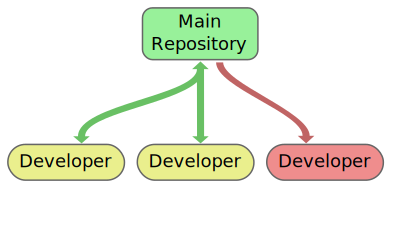
\includegraphics[width=\linewidth]{centralized.pdf}
%   \end{minipage}  
%   \begin{minipage}{0.48\linewidth}
%     \begin{itemize}
%       \item One central repository
%       \item Individual access rights
%       \item Examples: CVS, Subversion
%     \end{itemize}    
%   \end{minipage}  
% }

\subsection{Centralized vs. distributed Version Control Systems}
\begin{frame}[fragile]
  \frametitle{Centralized vs. distributed Version Control Systems}
  \begin{minipage}{0.45\linewidth}
    \begin{center}
      \textbf{Centralized Model}
    \end{center}
    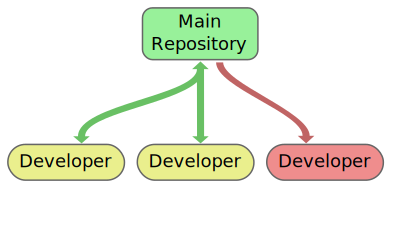
\includegraphics[width=\linewidth]{centralized.pdf}
    \begin{itemize}
      \item One central repository with individual access rights
      \item Changes apply immediately to all developers
      \item Examples: CVS, Subversion
    \end{itemize}
  \end{minipage}
  \textbf{vs.}
  \begin{minipage}{0.45\linewidth}
    \begin{center}
      \textbf{Distributed Model}
    \end{center}
    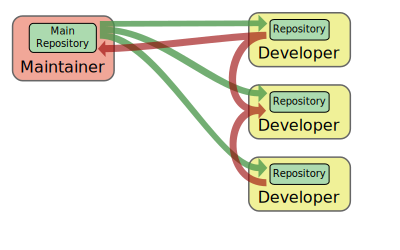
\includegraphics[width=\linewidth]{distributed.pdf}
    \begin{itemize}
      \item Each developer has his/her own local repository
      \item Changes can be shared between them
      \item Examples: Git, Mercurial
    \end{itemize}
  \end{minipage}
% 
%   \begin{minipage}{0.6\linewidth}
%     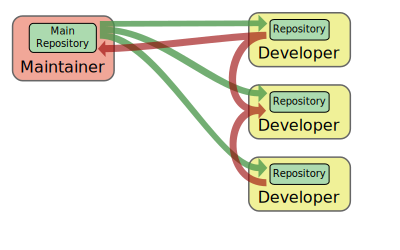
\includegraphics[width=\linewidth]{distributed.pdf}
%   \end{minipage}  
%   \begin{minipage}{0.38\linewidth}
%     \begin{itemize}
%       \item Every developer has its own repository
%       \item Each developer has read and write access to his/her own one
%       \item Share changes with other developers
%       \item Examples: Git, Bazaar, Monotone
%     \end{itemize}    
%   \end{minipage}  
\end{frame}

\subsection{Pros and cons of the distributed model}
\frame
{
  \frametitle{Pros and cons of the distributed model}
  \begin{block}{Pros}
    \begin{itemize}
      \item Don't need a connection to a network to work productively
      \item Some operations are much faster since no network is needed
      \item No sensitive single main repository
      \item Allow easy participation in project without permission
      \item Usually easier branching and merging
    \end{itemize}
  \end{block}
  \begin{block}{Cons}
    \begin{itemize}
      \item More complex concept
      \item No dedicated version at one time, no easy revision numbers
      \item No separated backup copy
    \end{itemize}
  \end{block}

}

\subsection{How to get Git}
\frame
{
  \frametitle{How to get Git}
  \begin{block}{POSIX}
    \begin{itemize}
      \item Official Homepage: \texttt{http://git-scm.com/}
      \item After the setup Git will be available on the command line
    \end{itemize}

  \end{block}
  \begin{block}{Windows}
    Under \texttt{http://nathanj.github.com/gitguide/} you can find a quick introduction about installing and using Git on Windows.\smallskip

    After the setup of \texttt{msysgit} (Windows port of Git) you can 
    \begin{itemize}
      \item Right click in your explorer and go to "Git Bash Here"
      \item A command line starts right in the current folder
      \item And now you can use all the commands given in this talk!
    \end{itemize}
  %to start a command line right in the current folder. Now you can use the same commands given in this talk!
    %\begin{itemize}
      %\item msysgit at \texttt{http://code.google.com/p/msysgit/}
      %\item After the setup a ``Git Bash'' (a special command line) will be avialable to work with Git
      %\item In the Explorer: Right click on a folder and go to "Git Bash Here" to open the Git Bash right in this folder
      %\item Now you can use the plain Git commands 
% TODO: Nice picture of Windows in action
    %\end{itemize}
  \end{block}
}
\section{Basic Concepts}
\subsection{Structure of a repository}
\begin{frame}
  \frametitle{Structure of a repository}
  A repository consists of several parts:
  \begin{minipage}{0.7\linewidth}
    \includegraphics<1>[width=\linewidth]{repo-history.pdf}  
    \includegraphics<2>[width=\linewidth]{repo-refs.pdf}
    \includegraphics<3>[width=\linewidth]{repo-worktree.pdf}
    \includegraphics<4>[width=\linewidth]{repo-index.pdf}
  \end{minipage}
  \begin{minipage}{0.27\linewidth}
    \begin{enumerate}
      \item<1-> Objects representing the history of the tracked content
      \item<2-> ``Refs,'' the reference
      \item<3-> Working tree
      \item<4-> Index/Stage
    \end{enumerate}
  \end{minipage}  
\end{frame}

\subsection{How can the objects in the history be adressed?}
\begin{frame}
  \frametitle{How can the objects in the history be adressed?}
  \begin{minipage}{0.33\linewidth}
    \includegraphics<1>[width=\linewidth]{objects.pdf}
    \includegraphics<2>[width=\linewidth]{objects-sha1.pdf}
    \includegraphics<3->[width=\linewidth]{objects-name.pdf}
  \end{minipage}  
  \begin{minipage}{0.6\linewidth}
    \begin{itemize}
      \item<1-> Every object in the history stores its type, size and content
      \item<2-> From this data the SHA1 hash (40-digit number) is calculated
      \item<3-> This value serves as a unique name. Collisions are highly unlikely!
    \end{itemize}    
  \end{minipage}
\end{frame}

\subsection{What do the objects in the history look like?}
\begin{frame}
  \frametitle{What do the objects in the history look like?}  
  \begin{minipage}[t]{0.5\linewidth}
    \only<1>{\large{Blob objects}\\}
    \only<2>{\large{Tree objects}\\}
    \only<3>{\large{Commit objects}\\}
    \only<4>{\large{Tag objects}\\}
    \includegraphics<1>[width=\linewidth]{history-with-objects-blob.pdf}  
    \includegraphics<2>[width=\linewidth]{history-with-objects-tree.pdf}  
    \includegraphics<3>[width=\linewidth]{history-with-objects-commit.pdf}  
    \includegraphics<4>[width=\linewidth]{history-with-objects-tag.pdf}  
  \end{minipage}
  \begin{minipage}[t]{0.48\linewidth}
    \only<1>{
      \begin{itemize}
        \item A blob object represents a file and contain the file's content
      \end{itemize}
    }
    \only<2>{
      \begin{itemize}
        \item A tree object represents a directory and its content
        \item It contains a list of SHA1 values pointing to other tree and blob objects
      \end{itemize}
    }
    \only<3>{
      \begin{itemize}
        \item A commit represents a snapshot of the working directory
        \item It contains the
          \begin{itemize}
            \item SHA1 of the corresponding tree object
            \item SHA1 of the parent commit
            \item Name of the author and the committer
            \item Message describing the commit
          \end{itemize}          
      \end{itemize}
    }
    \only<4>{
      \begin{itemize}
        \item A tag points out a certain object in your history
        \item It contains the
          \begin{itemize}
            \item SHA1 name of the tagged object and its type
            \item Name of the person who created the tag
            \item Message describing the tag
          \end{itemize}          
      \end{itemize}      
    }
  \end{minipage} 
\end{frame}

%~ \begin{frame}
  %~ \frametitle{An Example}
  %~ \begin{center}
    %~ 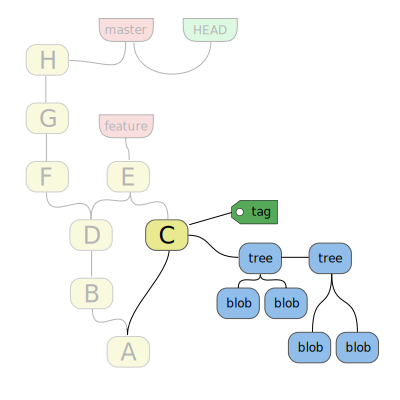
\includegraphics[width=0.5\linewidth]{history-with-objects.pdf}
  %~ \end{center}
%~ \end{frame}

\section{How to start}
\subsection{Basics}
\begin{frame}
  \frametitle{Basics}
  Every Git command looks like this\medskip
  
  {\tt\ \$ git [<options>] command [<options>]}\medskip
  
  \pause
  For example:\medskip
  
  {\tt\ \$ git --help commit}\\
  {\tt\ \$ git commit -m "Message"}\\
  {\tt\ \$ git-merge featureX}\medskip
  
  \pause
  There are
  \begin{itemize}
    \item ca. 140 commands
    \item ca. 25 every day commands
    \item 4 GUI commands
  \end{itemize}   
\end{frame}

\subsection{Where to get help?}
\begin{frame}
    \frametitle{Where to get help?}
    To get the most common Git commands\medskip
    
    {\tt\ \$ git --help}\medskip
   
    \pause
    Need help to a certain Git command\medskip
    
    {\tt\ \$ git --help command}\medskip
    
    \pause
    Two online books with many informations:
    \begin{itemize}
      \item The Git community book: \texttt{http://book.git-scm.com/}
      \item Pro Git book: \texttt{http://progit.org/book/}
    \end{itemize}
    Tips collections:
    \begin{itemize}
      \item Git ready: \texttt{http://gitready.com/}
      \item And of course: Your favorite online search engine
    \end{itemize}
\end{frame}

\subsection{Before you start}
\begin{frame}
  \frametitle{Before you start}
  \begin{itemize}
    \item You should set your name and email address\\
      {\tt\ \$ git config [--global] user.name <name>}\\
      {\tt\ \$ git config [--global] user.email <email>}
    \item<2-> Tell Git which editor you like to use (for example to edit the commit messages)
      {\tiny a.k.a to which religion do you belong?}\\
			{\tt\ \$ git config [--global] core.editor <editor>}
		\item<3-> To get a list of your settings\\
			{\tt\ \$ git config [--global] --list}
  \end{itemize}
  %~ %\vspace{-0.5ex}
  %~ \pause
  %~ \begin{minipage}{0.55\textwidth}
    %~ \begin{itemize}
      %~ \item Create a new repository\\
        %~ \begin{itemize}
          %~ \item Go to the directory whose content shall be in a repository and type
          %~ \item  {\tt\ \$ git init}
        %~ \end{itemize}
      %~ \pause
      %~ \item Clone an existing repository
        %~ \begin{itemize}
          %~ \item Go to the directory which shall contain the directory with the repository and type
          %~ \item {\tt\ \$ git clone <URL>}
        %~ \end{itemize}
    %~ \end{itemize}    
  %~ \end{minipage}
  %~ \pause[2] 
  %~ \begin{minipage}{0.4\linewidth}
    %~ \includegraphics<2>[width=\linewidth]{init.pdf}
    %~ \includegraphics<3>[width=\linewidth]{clone.pdf}
  %~ \end{minipage}  
\end{frame}

\subsection{Inspecting your Repository}
\begin{frame}
	\frametitle{Inspecting your Repository}
	\begin{minipage}{0.55\linewidth}
		\begin{itemize}
			\item To get the status of your working directory\\
				{\tt\ \$ git status}
			\item<2-> The changes between working tree and last commit\\
				{\tt\ \$ git diff HEAD}
			\item<3-> Review the last commit\\
				{\tt\ \$ git show HEAD}
			\item<4-> To inspect the history of the repository\\
				{\tt\ \$ git log}
			\item<5-> To see a nice tree of your history\\
				{\tt\ \$ gitk [--all]}\\
				{\tiny \texttt{--all} to show all branches}
		\end{itemize}	
	\end{minipage}
	\begin{minipage}{0.4\linewidth}
		\centering
		\includegraphics<1>[width=\linewidth]{status.pdf}
		\includegraphics<2>[width=\linewidth]{diff-head.pdf}
		\includegraphics<3>[width=\linewidth]{show.pdf}
		\includegraphics<4>[width=\linewidth]{log.pdf}
		\includegraphics<5>[width=\linewidth]{gitk-rails.jpg}
	\end{minipage}
\end{frame}

%~ \subsection{Inspecting your Repository}
%~ \begin{frame}
  %~ \frametitle{Inspecting your Repository I}
  %~ \framesubtitle{Show the current state of the repository}
  %~ \begin{minipage}{0.55\linewidth}
    %~ \begin{itemize}
      %~ \item Status of the current working tree\\
        %~ {\tt\ \$ git status}\\
      %~ \pause
      %~ \item Changes between index and working tree\\
        %~ {\tt\ \$ git diff}\\
      %~ \pause
      %~ \item Changes between index and last commit\\
        %~ {\tt\ \$ git diff --staged}\\
      %~ \pause
      %~ \item Changes between current working tree and last commit\\
        %~ {\tt\ \$ git diff HEAD}\bigskip
    %~ \end{itemize}
  %~ \end{minipage}
  %~ \pause[1]
  %~ \begin{minipage}{0.4\linewidth}
    %~ \centering
    %~ \includegraphics<1>[width=\linewidth]{status.pdf}
    %~ \includegraphics<2>[width=\linewidth]{diff.pdf}
    %~ \includegraphics<3>[width=\linewidth]{diff-staged.pdf}
    %~ \includegraphics<4>[width=\linewidth]{diff-head.pdf}
  %~ \end{minipage}  
%~ \end{frame}
%~ 
%~ \begin{frame}
  %~ \frametitle{Inspecting your Repository II}
  %~ \framesubtitle{Review commits}
  %~ \begin{minipage}{0.55\linewidth}
    %~ \begin{itemize}
      %~ \item Review the last commit\\
        %~ {\tt\ \$ git show}
      %~ \pause
      %~ \item Review parent commit of the last commit\\
        %~ {\tt\ \$ git show HEAD\textasciitilde 1}
      %~ \pause
      %~ \item Changes in the last commit\\
        %~ {\tt\ \$ git show --name-status}
      %~ \pause
      %~ \item Show contents of \texttt{<file>} in the last commit\\
        %~ {\tt\ \$ git show HEAD:<file>}\\
    %~ \end{itemize}
  %~ \end{minipage}
  %~ \pause[1]
  %~ \begin{minipage}{0.4\linewidth}
    %~ \centering
    %~ \includegraphics<1>[width=\linewidth]{show.pdf}
    %~ \includegraphics<2>[width=\linewidth]{show-before.pdf}
    %~ \includegraphics<3>[width=\linewidth]{show-name-status.pdf}
    %~ \includegraphics<4>[width=\linewidth]{show-file.pdf}
  %~ \end{minipage}\medskip
%~ 
  %~ \pause[4]
  %~ Remark: \texttt{HEAD\textasciitilde n} is the parent commit of \texttt{HEAD\textasciitilde (n-1)} (for $n>1$) and \texttt{HEAD\textasciitilde 1}\ =\ \texttt{HEAD\^} is the parent commit of the last commit.
%~ \end{frame}
%~ 
%~ \begin{frame}
  %~ \frametitle{Inspecting your Repository III}
  %~ \framesubtitle{Review the complete commit history}
  %~ \begin{minipage}{0.55\linewidth}
    %~ \begin{itemize}
      %~ \item See commit history\\
        %~ {\tt\ \$ git log}
      %~ \pause
      %~ \item See commit history from the next to last commit to the last one\\
        %~ {\tt\ \$ git log HEAD\textasciitilde 1..HEAD}
      %~ \pause
      %~ \item A nice tree of your history\\
        %~ {\tt\ \$ gitk [--all]}\\
        %~ {\tiny \texttt{--all} to show all branches}
    %~ \end{itemize}
  %~ \end{minipage}
  %~ \pause[1]
  %~ \begin{minipage}{0.4\linewidth}
    %~ \centering
    %~ \includegraphics<1>[width=\linewidth]{log.pdf}
    %~ \includegraphics<2>[width=\linewidth]{log-head.pdf}
    %~ \includegraphics<3>[width=\linewidth]{gitk-rails.jpg}
  %~ \end{minipage}  
%~ \end{frame}

\section{Git Workflow - Private Repository}
\subsection{Commit}
\begin{frame}
  \frametitle{Commit}
  \begin{minipage}{0.5\linewidth}
    \includegraphics<1>[width=\linewidth]{workflow-empty.pdf}
    \includegraphics<2>[width=\linewidth]{workflow-add.pdf}
    \includegraphics<3>[width=\linewidth]{workflow-commit.pdf}
    \includegraphics<4>[width=\linewidth]{workflow-next-add.pdf}
    \includegraphics<5>[width=\linewidth]{workflow-next-commit.pdf}
  \end{minipage}  
  \begin{minipage}{0.47\linewidth}
    \begin{itemize}
      \item Initialize Repository\\
        {\tt\ \$ git init}
      \pause
      \item Create/modify files and stage them\\
        {\tt\ \$ git add <files>}
      \pause
      \item Commit the staged items\\
        {\tt\ \$ git commit -m <msg>}
      \pause
      \item Create/modify other files and stage them\\
        {\tt\ \$ git add <files>}
      \pause
      \item Commit these staged items\\
        {\tt\ \$ git commit -m <msg>}
    \end{itemize}    
  \end{minipage}  
\end{frame}

\subsection{Branching}
\begin{frame}
  \frametitle{Branching}
  \begin{minipage}{0.5\linewidth}
    \includegraphics<1>[width=\linewidth]{workflow-branching.pdf}
    \includegraphics<2>[width=\linewidth]{workflow-switch.pdf}
    \includegraphics<3>[width=\linewidth]{workflow-branch-add.pdf}
    \includegraphics<4>[width=\linewidth]{workflow-branch-commit.pdf}
  \end{minipage}  
  \begin{minipage}{0.47\linewidth}
    \begin{itemize}
      \item<1-4> Create a new branch\\
        {\tt\ \$ git branch <name>}\\
        Inspect available branches\\
        {\tt\ \$ git branch}
      \item<2-4> Switch to a branch\\
        {\tt\ \$ git checkout <name>}
      \item<3-4> Create/modify files and stage them\\
        {\tt\ \$ git add <files>}
      \item<4> Commit them to the currently active branch\\
        {\tt\ \$ git commit -m <msg>}
    \end{itemize}    
  \end{minipage}  
\end{frame}

\subsection{Merging}
\begin{frame}
  \frametitle{Merging - the simple case}
  \begin{minipage}{0.5\linewidth}
    \includegraphics<1>[width=\linewidth]{workflow-branch-switch.pdf}
    \includegraphics<2->[width=\linewidth]{workflow-branch-ff-merge.pdf}
  \end{minipage}  
  \begin{minipage}{0.47\linewidth}
    \begin{itemize}
      \item Switch to a branch\\
        {\tt\ \$ git checkout <name>}
      \item<2-> Merge \texttt{<branch>} into current branch\\
        {\tt\ \$ git merge <branch>}
    \end{itemize}
    \pause[3]
    \centering\bf Fast forward merge!
  \end{minipage}  
\end{frame}

\begin{frame}
  \frametitle{Merging - the standard case}
  \begin{minipage}{0.5\linewidth}
    \includegraphics<1>[width=\linewidth]{workflow-branch-switch.pdf}
    \includegraphics<2>[width=\linewidth]{workflow-branch-new-add.pdf}
    \includegraphics<3>[width=\linewidth]{workflow-branch-new-commit.pdf}
    \includegraphics<4>[width=\linewidth]{workflow-branch-new-merge.pdf}
  \end{minipage}  
  \begin{minipage}{0.47\linewidth}
    \begin{itemize}
      \item Switch to a branch\\
        {\tt\ \$ git checkout <name>}
      \pause
      \item Create/modify files and stage them\\
        {\tt\ \$ git add <files>}
      \pause
      \item Commit staged items\\
        {\tt\ \$ git commit -m <msg>}
      \pause
      \item Merge \texttt{<branch>} into current branch\\
        {\tt\ \$ git merge <branch>}
    \end{itemize}
  \end{minipage}  
\end{frame}

\subsection{Merging conflicts}
\begin{frame}
  \frametitle{Merging conflicts}
  \begin{minipage}{0.5\linewidth}
    \includegraphics<1>[width=\linewidth]{workflow-branch-new-merge-conflict.pdf}
    \includegraphics<2->[width=\linewidth]{workflow-branch-new-merge-conflict-status.pdf}
  \end{minipage}  
  \begin{minipage}{0.47\linewidth}
    Merging conflicts occur if for example the same file differs at the same line in the two branches.\smallskip
    \pause
    
    After a failed merge the repository remains in a special state: 
    \begin{itemize}
      \item All well merged files are written to the index and the working directory
      \item The index contains all three versions of the unmerged file
      \item The working tree contains a special version of the unmerged file
    \end{itemize}
%    \pause
%    To resolve the conflict you have to
%    \begin{itemize}
%      \item Edit all conflicted files in your working directory
%      \item Add them to the index with \texttt{git add <file>}
%      \item Commit the current state of the index 
%    \end{itemize}    
  \end{minipage}  
\end{frame}

\begin{frame}
  \frametitle{Merging conflicts - file versions}
  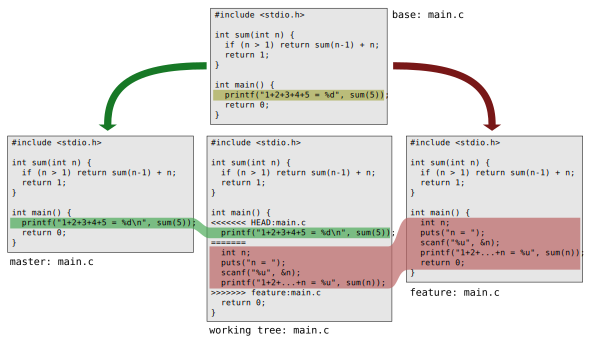
\includegraphics[width=\linewidth]{workflow-branch-new-merge-conflict-versions.pdf}
\end{frame}

\begin{frame}
  \frametitle{Merging conflicts - resolve conflict}
  \begin{minipage}{0.5\linewidth}
    \includegraphics<1>[width=\linewidth]{workflow-branch-new-merge-conflict-edit.pdf}
    \includegraphics<2>[width=\linewidth]{workflow-branch-new-merge-conflict-resolve.pdf}
    \includegraphics<3>[width=\linewidth]{workflow-branch-new-merge-conflict-resolve-commit.pdf}
  \end{minipage}  
  \begin{minipage}{0.47\linewidth}
    To resolve a merging conflict you have to
    \begin{itemize}
      \item<1-> Edit the unmerged files 
      \item<2-> Add the corrected files to the index\\
        {\tt\ \$ git add <files>}
      \item<3-> Complete the merge by commiting the index\\
%        \begin{itemize}
%          \item Automatically merged and added files (added by Git)
%          \item Manually corrected and added files (added by you)
%        \end{itemize}
        {\tt\ \$ git commit -m <msg>}
    \end{itemize}
%    \pause
%    To resolve the conflict you have to
%    \begin{itemize}
%      \item Edit all conflicted files in your working directory
%      \item Add them to the index with \texttt{git add <file>}
%      \item Commit the current state of the index 
%    \end{itemize}    
  \end{minipage}  
%Unless you haven't resolved the conflict Git doesn't allow any 
%  To resolve the conflict you have to
%  \begin{itemize}
%    \item Edit the unmerged files
%    \item Add the corrected files to the index\\
%      {\tt\ \$ git add <unmerged files>}
%    \item Complete the merge by commiting the index containing the
%      \begin{itemize}
%        \item Automatically merged and added files (added by Git)
%        \item Manually corrected and added files (added by you)
%      \end{itemize}
%      {\tt\ \$ git commit -m "<message>"}
%  \end{itemize}
\end{frame}

\subsection{Undo things}
\begin{frame}
  \frametitle{Undo things}
  \begin{minipage}{0.5\linewidth}
    \includegraphics<1>[width=\linewidth]{undo.pdf}
    \includegraphics<2>[width=\linewidth]{undo-revert.pdf}
    \includegraphics<3>[width=\linewidth]{undo-reset.pdf}
    \includegraphics<4>[width=\linewidth]{undo-revert-merge.pdf}
    \includegraphics<5>[width=\linewidth]{undo-revert-merge-1.pdf}
    \includegraphics<6>[width=\linewidth]{undo-revert-merge-2.pdf}
    \includegraphics<7>[width=\linewidth]{undo-restore-file.pdf}
  \end{minipage}  
  \begin{minipage}{0.47\linewidth}
    \begin{itemize}
      \item<2-> Revert \texttt{<commit>} by creating a new commit\\
        {\tt\ \$ git revert <commit>}
      \item<3-> Reset the \texttt{HEAD} to \texttt{<commit>}\\
        {\tt\ \$ git reset\\
         \qquad\lbrack--hard\textbar --soft\rbrack\\
         \qquad <commit>}\\
        {\tiny\texttt{--hard} to set all files to the new state}
      \item<4-> Revert a merge \texttt{<commit>}\\
        {\tt\ \$ git revert \\
         \quad -m <parent> <commit>}\\
        {\tiny\texttt{-m \textit{n}} denotes the $n$-th parent of the commit}
      \item<7-> Restore an individual file\\
        {\tt\ \$ git checkout\\
         \qquad<ref> <file>}
    \end{itemize}
  \end{minipage}  
\end{frame}

\section{Git Workflow - share your code with others}
\subsection{Remote repositories}
\begin{frame}
  \frametitle{Remote repositories}
  A remote repository is a repository which at least partly shares the same history with yours.
  \begin{itemize}
    \item List all remotes\\
      {\tt\ \$ git remote [-v]}
    \item Show details about a given remote\\
      {\tt\ \$ git remote show <name>}
    \item Add a new remote repository located at \texttt{<URL>}\\
      {\tt\ \$ git remote add <name> <URL>}
    \item Remove a given remote\\
      {\tt\ \$ git remote rm <name>}
  \end{itemize}
\end{frame}

\subsection{Clone an existing repository}
\begin{frame}
  \frametitle{Clone an existing repository}
  \begin{minipage}{0.5\linewidth}
    \includegraphics<1>[width=\linewidth]{remote.pdf}
    \includegraphics<2>[width=\linewidth]{remote-clone.pdf}
  \end{minipage}
  \begin{minipage}{0.47\linewidth}
    \begin{itemize}
      \item<2-> Clone a repository\\
        {\tt\ \$ git clone <URL>}
        \begin{itemize}
          \item All objects from the repository are downloaded
          \item But only currently active branch of the remote will be checked out as a branch
          \item Remote branches to all other branches
        \end{itemize}
        {\tiny }
    \end{itemize}
  \end{minipage}  
\end{frame}

\subsection{Pulling from a remote}
\begin{frame}
  \frametitle{Pulling from a remote - The safe procedure}
  \begin{minipage}{0.5\linewidth}
    \includegraphics<1>[width=\linewidth]{remote-clone.pdf}
    \includegraphics<2>[width=\linewidth]{remote-commits.pdf}
    \includegraphics<3>[width=\linewidth]{remote-fetch.pdf}
    \includegraphics<4>[width=\linewidth]{remote-checkout-remote.pdf}
  \end{minipage}
  \begin{minipage}{0.47\linewidth}
    \begin{itemize}
      \item<2-4> Commits to the remote and your repository (worst case scenario)
      \item<3-4> Fetch newest changes\\
        {\tt\ \$ git fetch <remote>}
        \begin{itemize}
          \item Objects will be loaded down but not merged
          \item Remote branches are updated
        \end{itemize}
      \item<4-4> Create a new branch tracking a remote branch and check it out\\
        {\tt\ \$ git checkout -b\\
         \quad\ <name> <rem-branch>}
      \item<4-4> Test the changes thoroughly!
      
    \end{itemize}
  \end{minipage}  
\end{frame}

%\subsection{Pulling from a remote }
\begin{frame}
  \frametitle{Pulling from a remote - The safe procedure}
  \begin{minipage}{0.5\linewidth}
    \includegraphics<1>[width=\linewidth]{remote-merge.pdf}
    \includegraphics<2->[width=\linewidth]{remote-delete.pdf}
  \end{minipage}
  \begin{minipage}{0.47\linewidth}
    \begin{itemize}
    \item<1->commit your changes to {\tt<name>} in case you changed something
    \end{itemize}
    If you agree to the changes:
    \begin{itemize}
      \item<2-> Merge the changes to the \texttt{master} branch\\
        {\tt\ \$ git checkout master}\\
        {\tt\ \$ git merge <branch>}
      \item<3-> Delete the temporary \texttt{test} branch\\
        {\tt\ \$ git branch (-d|-D)\\
         \quad\ <branch>}\\
        {\tiny \texttt{-d} checks whether the branch is already merged}
    \end{itemize}
  \end{minipage}
\end{frame}

\begin{frame}
  \frametitle{Pulling from a remote}
  If you always agree to the changes in the remote, use\smallskip
  
    {\tt\ \$ git pull <remote> [<branch>]}\smallskip
    
  to fetch the changes from \texttt{<remote>} and merge them right into your repository.
\end{frame}

\subsection{Pushing to a remote}
\begin{frame}
  \frametitle{Pushing to a remote}
  \begin{minipage}{0.5\linewidth}
    \includegraphics<1>[width=\linewidth]{remote-want-to-push-simple.pdf}
    \includegraphics<2>[width=\linewidth]{remote-push-simple.pdf}
  \end{minipage}
  \begin{minipage}{0.47\linewidth}
    You want to
    \begin{itemize}
     \item Update a remote repository,
     \item That \alert{did not} change until your last local modifications
    \end{itemize} 
    \pause 
    then you can
    \begin{itemize}
      \item<2-> Push the changes to the remote\\
        {\tt\ \$ git push <remote>\\
         \qquad [<branch>]}\\
        {\tiny No \texttt{<branch>} given: Updates all matching branches}
    \end{itemize}
  \end{minipage}  
\end{frame}

\subsection{Pushing to a remote}
\begin{frame}
  \frametitle{Pushing to a remote}
  \begin{minipage}{0.5\linewidth}
    \includegraphics<1>[width=\linewidth]{remote-want-to-push-problem.pdf}
    \includegraphics<2>[width=\linewidth]{remote-pull-problem.pdf}
    \includegraphics<3>[width=\linewidth]{remote-push-problem.pdf}
  \end{minipage}
  \begin{minipage}{0.47\linewidth}
    You want to
    \begin{itemize}
     \item Update a remote repository,
     \item That \alert{did} change until your last local modifications
    \end{itemize} 
    then you can't simply push!
    \begin{itemize}
      \item<2-> Pull the changes into your repository\\
        {\tt\ \$ git pull <remote> \\
         \qquad [<branch>]}\\
        {\tiny No \texttt{<branch>} given: Updates all matching branches}
      \item<3-> Push your updated repository to the remote\\
        {\tt\ \$ git push <remote> \\
         \qquad [<branch>]}
    \end{itemize}
  \end{minipage}  
\end{frame}

%\subsection{Basic commands II}
%\begin{frame}
%  \frametitle{Basic commands II}
%  \begin{block}{}
%    \texttt{\$ git config --global user.name <name>}\\
%    \texttt{\$ git config --global user.email <youremail>}
%  \end{block}
%  \begin{block}{Create a new repository}
%    \begin{enumerate}
%      \item Go to the directory whose content shall be in a repository
%      \item \texttt{\$ git init}
%    \end{enumerate} 
%  \end{block}
%  \begin{block}{Clone an existing repository}
%    \begin{enumerate}
%      \item Go to directory which shall contain the directory with the repository
%      \item \texttt{\$ git clone <URL>}
%    \end{enumerate} 
%  \end{block}
%\end{frame}

%Git is strongly influenced by other distributed VCS like BitKeeper or Monotone. 
%Linus state some criteria for the next 
%However all of them don't meet all some of the following criteria 
%  \begin{tabular}{|l|l|l|}
%    \hline
%    Model & Centralized & Distributed \\
%    \hline\hline
%    Examples & CVS, Subversion & Mercurial, Monotone, Git, ... \\
%    Illustration & 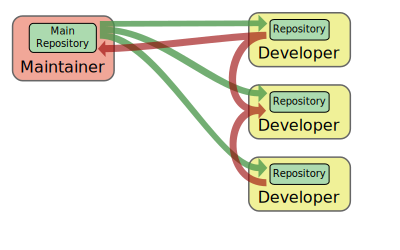
\includegraphics[width=0.3\linewidth]{distributed.pdf}
%  \end{tabular}

%\subsection{Overview of the Beamer Class}
%\frame
%{
%  \frametitle{Features of the Beamer Class}
%
%  \begin{itemize}
%  \item<1-> Normal LaTeX class.
%  \item<2-> Easy overlays.
%  \item<3-> No external programs needed.      
%  \end{itemize}
%}
\section{How to remember all this stuff?}
\subsection{Git cheat sheet}
\begin{frame}
  \frametitle{Git cheat sheet}
  Gives you an overview of all important Git commands
  \begin{center}
    \frame{\includegraphics[scale=0.25]{git-cheat-sheet.pdf}}
  \end{center}
  Download and print it and nail it onto the wall at your desk!
\end{frame}

\begin{frame}
  \begin{center}{}
    \begin{LARGE}
      Thank you for your attention!
    \end{LARGE}
  \end{center}\bigskip

You can get this talk by using Git: Just type\smallskip

\quad\texttt{git clone git://github.com/waehnert/gittalk.git}\smallskip

to get a copy of the talk.
\end{frame}

\section*{Additional Information}
\subsection*{Public repositories}
\begin{frame}
  \frametitle{Public repositories}
  \begin{minipage}{0.5\linewidth}
    \includegraphics<1>[width=\linewidth]{public-repos-own.pdf}
    \includegraphics<2>[width=\linewidth]{public-repos-own-rw.pdf}
    \includegraphics<3>[width=\linewidth]{public-repos-main.pdf}
    \includegraphics<4>[width=\linewidth]{public-repos-main-pull.pdf}
    \includegraphics<5>[width=\linewidth]{public-repos-upload.pdf}
  \end{minipage}
  \begin{minipage}{0.47\linewidth}
    \begin{itemize}
      \item<1-> Each developer has its own private and public repository
      \item<2-> You can pull from and push to your public repository
      \item<3-> Among these repositories there is the main repository
      \item<4-> Every developer can pull the newest official changes from this main repository
      \item<5-> Now each developer works on the project and makes the changes publicly available
    \end{itemize}
  \end{minipage}
\end{frame}

\begin{frame}
  \frametitle{Public repositories}
  \begin{minipage}{0.5\linewidth}
    \includegraphics<1>[width=\linewidth]{public-repos-share.pdf}
    \includegraphics<2>[width=\linewidth]{public-repos-bringin.pdf}
    \includegraphics<3>[width=\linewidth]{public-repos-main-pull.pdf}
  \end{minipage}
  \begin{minipage}{0.47\linewidth}
    \begin{itemize}
      \item<1-> The developers can share changes among each other
      \item<2-> If you want to bring your changes into the main repository you have to make a pull request to its
        maintainer
      \item<3-> If these changes are accepted they can be pulled by others from the main repository
    \end{itemize}
  \end{minipage}
\end{frame}

\subsection*{Short History}
\begin{frame}
  \frametitle{Short History}
  \begin{description}
    \item[1991-2002] Changes to the Linux kernel were passed around as patches and archived files
    \item[2002-2005] The kernel project used the proprietary BitKeeper VCS
    \item[2005] The relation between the kernel community and BitMover Inc. broke down
    \item[Apr 3, 2005] Begin of the development of Git as a replacement for BitKeeper
    \item[Feb 13, 2010] Release of the version 1.7.0
  \end{description}
\end{frame}

\subsection*{Design Goals}
\begin{frame}
  \frametitle{Design Goals}
  \begin{block}{Linus Torvalds had several design criteria}
    \begin{enumerate}
      \item Something opposite to CVS (Linus: "[...] and I hate it with passion.")
      \item Distributed version control system
      \item Strong safeguards against corruption, either accidental or malicious
      \item High performance
    \end{enumerate}
    Every VCS which existed in 2005 didn't meet at least one of these criteria. So Linus sat down and started writing Git.
  \end{block}

  \begin{small}
    Why ``Git''? Linus: ``I'm an egotistical bastard, and I name all my projects after myself. First Linux, now git.''\\
    \tiny a git, brit. en., stupid or unpleasant person
  \end{small}
\end{frame}

\subsection*{Basic Tagging}
\begin{frame}
  \frametitle{Basic Tagging}
  Tags are pointers to specific objects in your history.
  \begin{itemize}
    %\item To create a lightweight tag, i.e. without any description or information of its author\\
    %  {\tt\ \$ git tag <tag-name> [<object>]}
    \item To create an annotated tag containing a description and information about its author\\
      {\tt\ \$ git tag -a <tag-name> -m <msg> [<objects>]}
    \item To get the informations stored along with a tag\\
      {\tt\ \$ git show <tag-name>}
    \item To get a list of the available tags\\
      {\tt\ \$ git tag [-l <search-pattern>]}
    \item To delete a given tag (Public available tags shouldn't be deleted!)\\
      {\tt\ \$ git tag -d <name>}
      %{\tiny }
    \item To push a tag to a remote (Tags aren't transfered automaticaly!)\\
      {\tt\ \$ git push <remote> <tag>}
  \end{itemize}
\end{frame}


\end{document}
